\subsection{Pengujian sistem}
\label{subsection:pengujian-sistem}

Pengujian sistem dilakukan untuk memastikan bahwa sistem yang telah diimplementasikan berfungsi sesuai dengan yang diharapkan. Kebutuhan dari sistem dapat dilihat pada bagian \ref{tab:functional-requirements} dan bagian \ref{tab:non-functional-requirements}. Pengujian akan merujuk pada kebutuhan fungsional dan non-fungsional untuk spesifikasi perilaku sistem yang diharapkan. Untuk memudahkan pemetaan dan memastikan semua pengujian telah mencakup semua kebutuhan, lampiran \ref{appendix:pemetaan-pengujian} menyediakan tabel yang memetakan kebutuhan fungsional dan non-fungsional ke pengujian yang dilakukan.

\subsubsection{Pengujian operasi dasar}
\label{subsubsection:pengujian-operasi-dasar}

Pengujian ini mencakup fungsional F-1, yaitu bahwa sistem harus dapat melakukan operasi \textit{read} dan \textit{write} pada sebuah \textit{key-value store database}. Pengujian dibagi dua menjadi pengujian operasi \textit{write} dan \textit{read}. Kode dari pengujian tersebut adalah P-1 dan P-2. Pengujian ini menggunakan \textit{script} pembantu oneshot.js yang sudah dijelaskan pada Bagian \ref{subsubsection:implementasi-benchmark}.

Pengujian operasi \textit{write} dengan kode pengujian P-1 dilakukan dengan skenario pengguna menuliskan \textit{key-value pair} ke dalam sistem. Nilai \textit{key} dan \textit{value} akan bersifat acak. Berikut langkah-langkah yang dilakukan dalam pengujian ini:

\begin{enumerate}
	\item Menunggu hingga sistem siap menerima \textit{request}. Konfirmasi dapat dilakukan dengan mengirim \textit{request} HTTP pada \textit{endpoint} /status dan memastikan bahwa sistem sudah memiliki \textit{leader}.
	\item Menjalankan \textit{script} oneshot.js dengan argumen \textit{write} untuk melakukan pengujian operasi dasar. \textit{Script} ini akan mengirimkan \textit{request} \textit{write} ke sistem.
	\item Mengirim request HTTP pada \textit{endpoint} /log untuk memastikan bahwa sistem telah menerima \textit{request} \textit{write} dan telah menyimpan data yang dituliskan.
	\item Mengulangi pengujian dengan sistem \textit{erasure coding} dan juga dengan sistem replikasi.
\end{enumerate}

Hasil yang diharapkan setelah tes dijalankan adalah sistem menyimpan \textit{log} yang berisi \textit{key-value pair} yang telah dituliskan. Untuk \textit{erasure coding}, log yang disimpan harus berisi \textit{key-value pair} yang telah di-\textit{encode} sesuai dengan konfigurasi serta berbeda-beda untuk setiap \textit{node} sesuai dengan index \textit{fragment} yang diterima.

Pengujian operasi \textit{read} dengan kode pengujian P-2 dilakukan dengan skenario pengguna membaca \textit{key-value pair} yang sudah dituliskan sebelumnya. Berikut langkah-langkah yang dilakukan dalam pengujian ini:

\begin{enumerate}
	\item Menunggu hingga sistem siap menerima \textit{request}. Konfirmasi dapat dilakukan dengan mengirim \textit{request} HTTP pada \textit{endpoint} /status dan memastikan bahwa sistem sudah memiliki \textit{leader}.
	\item Menjalankan \textit{script} oneshot.js dengan argumen \textit{read} untuk melakukan pengujian operasi dasar. \textit{Script} ini akan mengirimkan \textit{request} \textit{read} ke sistem.
	\item Mengirim request HTTP pada \textit{endpoint} /log untuk memastikan bahwa sistem mengembalikan nilai \textit{request} \textit{read} yang sesuai dengan nilai yang disimpan pada \textit{log}.
	\item Mengulangi pengujian dengan sistem \textit{erasure coding} dan juga dengan sistem replikasi.
\end{enumerate}

Hasil yang diharapkan setelah tes dijalankan adalah sistem mengembalikan nilai \textit{key-value pair} yang telah dituliskan sebelumnya. Untuk \textit{erasure coding}, sistem harus dapat mengembalikan nilai \textit{key-value pair} yang utuh dan bukan nilai \textit{fragment} yang di-\textit{encode}.
\subsubsection{Pengujian penyimpanan data persistent}
\label{subsubsection:pengujian-penyimpanan-data-persistent}

Pengujian ini mencakup fungsional F-2, yaitu bahwa sistem harus dapat menyimpan data secara persistent pada \textit{key-value store database}. Pengujian dilakukan dengan kode pengujian P-3. Pengujian ini menggunakan \textit{script} pembantu oneshot.js yang sudah dijelaskan pada bagian \ref{subsubsection:implementasi-benchmark}.

Pengujian penyimpanan data \textit{persistent} dengan kode pengujian P-3 dilakukan dengan menuliskan \textit{key-value pair} ke dalam sistem, kemudian mematikan sistem, menyalakan kembali sistem dengan flag --continue, dan memastikan bahwa data yang dituliskan sebelumnya masih dapat diterima. Berikut langkah-langkah yang dilakukan dalam pengujian ini:

\begin{enumerate}
  \item Menunggu hingga sistem siap menerima \textit{request}. Konfirmasi dapat dilakukan dengan mengirim \textit{request} HTTP pada \textit{endpoint} /status dan memastikan bahwa sistem sudah memiliki \textit{leader}.
  \item Menjalankan \textit{script} oneshot.js dengan argumen \textit{write} untuk melakukan pengujian operasi dasar. \textit{Script} ini akan mengirimkan \textit{request} \textit{write} ke sistem.
  \item Mengirim request HTTP pada \textit{endpoint} /log untuk memastikan bahwa sistem telah menerima \textit{request} \textit{write} dan telah menyimpan data yang dituliskan.
  \item Mematikan sistem dengan menggunakan perintah stop\_all pada file scripts.sh.
  \item Menyalakan ulang sistem dengan menggunakan perintah run\_all pada file scripts.sh dengan tambahan flag --continue. Flag ini akan membuat sistem tidak menghapus data persisten yang sudah ada sebelumnya.
  \item Menjalankan \textit{script} oneshot.js dengan argumen \textit{read} untuk melakukan pengujian operasi dasar. \textit{Script} ini akan mengirimkan \textit{request} \textit{read} ke sistem.
  \item Mengirim request HTTP pada \textit{endpoint} /log untuk memastikan bahwa sistem mengembalikan nilai \textit{request} \textit{read} yang sesuai dengan nilai yang disimpan pada \textit{log}.
  \item Mengulangi pengujian dengan sistem \textit{erasure coding} dan juga dengan sistem replikasi.
\end{enumerate}

Hasil yang diharapkan setelah tes dijalankan adalah sistem mengembalikan nilai \textit{key-value pair} yang telah dituliskan sebelumnya. Untuk \textit{erasure coding}, sistem harus dapat mengembalikan nilai \textit{key-value pair} yang utuh dan bukan nilai \textit{fragment} yang di-\textit{encode}. Pengujian ini memastikan bahwa data yang disimpan pada sistem tetap ada meskipun sistem dimatikan dan dinyalakan kembali.
\subsubsection{Pengujian pencatatan waktu transaksi}
\label{subsubsection:pengujian-pencatatan-waktu-transaksi}

Pengujian ini mencakup fungsional F-3, yaitu bahwa sistem harus dapat mencatat waktu transaksi dari \textit{request} masuk hingga operasi selesai. Pengujian dibagi dua menjadi pengujian pencatatan waktu transaksi untuk operasi \textit{write} dan operasi \textit{read}. Kode dari pengujian tersebut adalah P-4 dan P-5. Pengujian ini menggunakan \textit{script} pembantu oneshot.js yang sudah dijelaskan pada bagian \ref{subsubsection:implementasi-benchmark}.

Pengujian pencatatan waktu transaksi dengan kode pengujian P-4 dilakukan dengan skenario pengguna mengirimkan \textit{request} \textit{write} ke sistem. Pengujian dilakukan dengan langkah-langkah sebagai berikut:

\begin{enumerate}
  \item Melakukan setup sistem menggunakan \textit{flag} --trace dan --file\_output seperti yang dijelaskan pada bagian \ref{subsection:setup-pengujian}.
  \item Menunggu hingga sistem siap menerima \textit{request}. Konfirmasi dapat dilakukan dengan mengirim \textit{request} HTTP pada \textit{endpoint} /status dan memastikan bahwa sistem sudah memiliki \textit{leader}.
  \item Menjalankan \textit{script} oneshot.js dengan argumen \textit{write} untuk melakukan pengujian operasi dasar. \textit{Script} ini akan mengirimkan \textit{request} \textit{write} ke sistem.
  \item Mengecek \textit{log} yang dihasilkan oleh sistem pada file \textit{output log} dan memastikan bahwa sistem mencatat waktu transaksi.
  \item Mengulangi pengujian dengan sistem \textit{erasure coding} dan juga dengan sistem replikasi.
\end{enumerate}

Hasil yang diharapkan adalah sistem menghasilkan \textit{log} yang memiliki informasi waktu setiap fungsi yang dipanggil dalam sebuah \textit{request} dari masuk hingga selesai. Contoh bentuk \textit{log} yang dihasilkan dapat dilihat pada gambar \ref{fig:log-trace}.

\begin{figure}[ht]
    \centering
    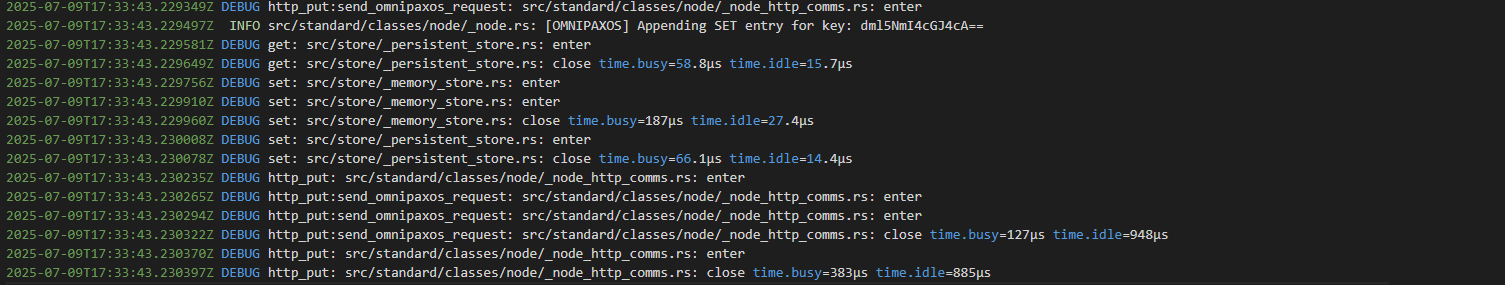
\includegraphics[width=0.95\textwidth]{resources/chapter-4/log-trace.png}
    \caption{Contoh log yang dihasilkan oleh sistem}
    \label{fig:log-trace}
\end{figure}

Pengujian pencatatan waktu transaksi dengan kode pengujian P-5 dilakukan dengan skenario pengguna mengirimkan \textit{request} \textit{read} ke sistem. Pengujian dilakukan dengan langkah-langkah sebagai berikut:

\begin{enumerate}
  \item Melakukan setup sistem menggunakan \textit{flag} --trace dan --file\_output seperti yang dijelaskan pada bagian \ref{subsection:setup-pengujian}.
  \item Menunggu hingga sistem siap menerima \textit{request}. Konfirmasi dapat dilakukan dengan mengirim \textit{request} HTTP pada \textit{endpoint} /status dan memastikan bahwa sistem sudah memiliki \textit{leader}.
  \item Menjalankan \textit{script} oneshot.js dengan argumen \textit{read} untuk melakukan pengujian operasi dasar. \textit{Script} ini akan mengirimkan \textit{request} \textit{read} ke sistem.
  \item Mengecek \textit{log} yang dihasilkan oleh sistem pada file \textit{output log} dan memastikan bahwa sistem mencatat waktu transaksi.
  \item Mengulangi pengujian dengan sistem \textit{erasure coding} dan juga dengan sistem replikasi.
\end{enumerate}

Hasil yang diharapkan adalah sistem menghasilkan \textit{log} yang memiliki informasi waktu setiap fungsi yang dipanggil dalam sebuah \textit{request} dari masuk hingga selesai. Contoh bentuk \textit{log} yang dihasilkan mirip dengan gambar \ref{fig:log-trace} dengan perbedaan pada \textit{request} yang dikirim adalah \textit{read}.
\subsubsection{Pengujian encoding data menggunakan erasure coding}
\label{subsubsection:pengujian-encoding-data-erasure-coding}

\subsubsection{Pengujian rekonstruksi data}
\label{subsubsection:pengujian-rekonstruksi-data}

Pengujian ini mencakup fungsional F-5, yaitu bahwa sistem harus dapat merekonstruksi data dari data yang disimpan menggunakan \textit{erasure coding}. Pengujian dilakukan dengan kode pengujian P-7. Pengujian ini menggunakan \textit{script} pembantu oneshot.js yang sudah dijelaskan pada bagian \ref{subsubsection:implementasi-benchmark}. Pengujian ini dilakukan dengan menuliskan \textit{key-value pair} ke dalam sistem lalu melakukan operasi \textit{read} pada \textit{key-value pair} tersebut untuk memastikan bahwa data yang disimpan telah di-\textit{encode} sesuai dengan konfigurasi yang telah ditentukan dan dapat direkonstruksi.

Pengujian rekonstruksi data dengan kode pengujian P-7 dilakukan dengan langkah-langkah sebagai berikut:
\begin{enumerate}
  \item Menunggu hingga sistem siap menerima \textit{request}. Konfirmasi dapat dilakukan dengan mengirim \textit{request} HTTP pada \textit{endpoint} /status dan memastikan bahwa sistem sudah memiliki \textit{leader}.
  \item Menjalankan \textit{script} oneshot.js dengan argumen \textit{write} untuk melakukan pengujian operasi dasar. \textit{Script} ini akan mengirimkan \textit{request} \textit{write} ke sistem.
  \item Mengirim \textit{request} HTTP pada \textit{endpoint} /fragment untuk memastikan bahwa sistem telah menerima \textit{request} \textit{write} dan telah menyimpan data yang dituliskan dalam bentuk \textit{fragment} yang telah di-\textit{encode}.
  \item Mengirim \textit{request} HTTP pada \textit{endpoint} /read untuk memastikan bahwa sistem dapat mengembalikan nilai \textit{key-value pair} yang telah di-\textit{encode} sesuai dengan konfigurasi yang telah ditentukan.
\end{enumerate}

Hasil yang diharapkan setelah tes dijalankan adalah sistem mengembalikan nilai \textit{key-value pair} yang telah dituliskan sebelumnya. Sistem harus dapat mengembalikan nilai \textit{key-value pair} yang utuh dan bukan nilai \textit{fragment} yang di-\textit{encode}.

Selain pengujian yang dilakukan dengan kode P-7, pengujian untuk kebutuhan fungsional F-4 juga dilakukan dengan \textit{automated testing} pada \textit{test suite} repository OmniPaxos. Pengujian yang dilakukan pada \textit{test suite} tersebut mengetes implementasi \textit{Erasure Coding Service} yang dibuat terlepas dari sistem \textit{key-value store database}.
\subsubsection{Pengujian distribusi data}
\label{subsubsection:pengujian-distribusi-data}

Pengujian ini mencakup fungsional F-5, yaitu bahwa sistem harus dapat mendistribusikan data atau sebagian data ke \textit{node} lain untuk keperluan ketahanan data. Pengujian dilakukan dengan kode pengujian P-8. Pengujian ini menggunakan \textit{script} pembantu oneshot.js yang sudah dijelaskan pada bagian \ref{subsubsection:implementasi-benchmark}. Pengujian ini dilakukan dengan menuliskan \textit{key-value pair} ke dalam sistem. Setelah itu, dilakukan melakukan \textit{request} GET ke \textit{endpoint} /fragment ke beberapa node lain untuk sistem \textit{erasure coding} dan \textit{endpoint} /read untuk sistem replikasi. Hal ini untuk memastikan bahwa data yang disimpan telah didistribusikan ke \textit{node} lain sesuai dengan konfigurasi yang telah ditentukan.

Pengujian distribusi data dengan kode pengujian P-8 dilakukan dengan langkah-langkah sebagai berikut:
\begin{enumerate}
    \item Menunggu hingga sistem siap menerima \textit{request}. Konfirmasi dapat dilakukan dengan mengirim \textit{request} HTTP pada \textit{endpoint} /status dan memastikan bahwa sistem sudah memiliki \textit{leader}.
    \item Menjalankan \textit{script} oneshot.js dengan argumen \textit{write} untuk melakukan pengujian operasi dasar. \textit{Script} ini akan mengirimkan \textit{request} \textit{write} ke sistem.
    \item Mengirim \textit{request} HTTP pada \textit{endpoint} /fragment ke beberapa \textit{node} lain untuk memastikan bahwa sistem telah mendistribusikan data yang dituliskan dalam bentuk \textit{fragment} yang telah di-\textit{encode}. Untuk sistem replikasi, mengirim \textit{request} HTTP pada \textit{endpoint} /read ke beberapa \textit{node} lain untuk memastikan bahwa sistem telah mendistribusikan data yang dituliskan ke \textit{node} lain.
    \item Mengirim \textit{request} HTTP pada \textit{endpoint} /read untuk memastikan bahwa sistem dapat mengembalikan nilai \textit{key-value pair} yang telah didistribusikan ke \textit{node} lain.
\end{enumerate}

Hasil yang diharapkan setelah tes dijalankan adalah sistem mengembalikan nilai \textit{key-value pair} yang telah didistribusikan. Untuk sistem \textit{erasure coding}, sistem harus dapat mengembalikan nilai \textit{key-value pair} yang berbentuk \textit{fragment} ter-\textit{encode}. Untuk sistem replikasi, sistem harus dapat mengembalikan nilai \textit{key-value pair} yang utuh.
\subsubsection{Pengujian konfigurasi sistem}
\label{subsubsection:pengujian-konfigurasi-sistem}

Pengujian ini mencakup fungsional F-7, yaitu bahwa sistem harus dapat dikonfigurasi untuk menggunakan \textit{erasure coding} atau replikasi tanpa mengganti konfigurasi lainnya. Pengujian dilakukan dengan kode pengujian P-9. Pengujian ini mencakup proses menjalankan sistem dengan konfigurasi yang sama dengan \textit{flag} tambahan --erasure dan tanpa \textit{flag} tersebut seperti yang sudah dijelaskan pada bagian \ref{subsection:setup-pengujian}.

Pengujian konfigurasi sistem dengan kode pengujian P-9 dilakukan dengan langkah-langkah sebagai berikut:
\begin{enumerate}
  \item Menyalakan sistem dengan konfigurasi \textit{erasure coding} menggunakan \textit{flag} --erasure. Konfirmasi dapat dilakukan dengan mengirim \textit{request} HTTP pada \textit{endpoint} /status dan memastikan bahwa sistem sudah memiliki \textit{leader}.
  \item Mematikan sistem dengan menggunakan perintah stop\_all pada file scripts.sh.
  \item Menyalakan ulang sistem tanpa \textit{flag} --erasure. Konfirmasi dapat dilakukan dengan mengirim \textit{request} HTTP pada \textit{endpoint} /status dan memastikan bahwa sistem sudah memiliki \textit{leader}.
\end{enumerate}

Hasil yang diharapkan setelah tes dijalankan adalah sistem dapat berjalan dengan konfigurasi \textit{erasure coding} dan juga dapat berjalan tanpa \textit{flag} tersebut. Tujuannya adalah untuk memastikan bahwa sistem dapat berjalan dengan konfigurasi yang sama dan hanya berbeda pada penggunaan \textit{erasure coding} atau replikasi.
\subsubsection{Pengujian perubahan konfigurasi ketahanan sistem}
\label{subsubsection:pengujian-perubahan-konfigurasi-ketahanan}
\subsubsection{Pengujian Request dengan Ukuran Data bervariasi}
\label{subsubsection:pengujian-request-ukuran-data}

Pengujian ini mencakup fungsional F-9, yaitu bahwa sistem harus dapat mensimulasikan \textit{request} dengan ukuran data yang bervariasi. Pengujian ini dilakukan dengan kode pengujian P-11.

Pengujian request dengan ukuran data bervariasi dengan kode pengujian P-11 dilakukan melalui mengatur variabel \textit{size} dan menjalankan perintah run\_bench\_suite pada file scripts.sh yang sudah dijelaskan pada bagian \ref{subsection:setup-pengujian}. Berikut langkah-langkah yang dilakukan dalam pengujian ini:

\begin{enumerate}
    \item Menunggu hingga sistem siap menerima \textit{request}. Konfirmasi dapat dilakukan dengan mengirim \textit{request} HTTP pada \textit{endpoint} /status dan memastikan bahwa sistem sudah memiliki \textit{leader}.
    \item Mengatur variabel \textit{size} pada file scripts.js dengan ukuran data yang bervariasi. Variabel ini menentukan seberapa besar data yang akan disimpan dalam sistem.
    \item Menjalankan perintah run\_bench\_suite pada file scripts.sh untuk menjalankan pengujian dengan ukuran data yang telah ditentukan.
\end{enumerate}

Hasil yang diharapkan setelah tes dijalankan adalah sistem dapat memulai \textit{benchmark} dengan \textit{request} dengan ukuran data yang bervariasi secara otomatis. Perlu dipastikan juga dalam penjalanan run\_bench\_suite tidak terdapat balikan \textit{error} dari sistem.
\subsubsection{Pengujian pengumpulan data}
\label{subsubsection:pengujian-pengumpulan-data}

Pengujian ini mencakup fungsional F-10, yaitu bahwa sistem harus dapat menjalankan \textit{request} secara berulang kali dan bervariasi secara otomatis untuk pengumpulan data. Pengujian dilakukan dengan kode pengujian P-12. Pengujian dilakukan dengan menjalankan perintah run\_bench\_suite pada file scripts.sh yang sudah dijelaskan pada bagian \ref{subsection:setup-pengujian}. Setelah itu dilakukan verifikasi dari durasi \textit{benchmark} yang dilakukan bahwa sistem menerima \textit{request} secara berulang kali.

Pengujian pengumpulan data dengan kode pengujian P-12 dilakukan dengan langkah-langkah sebagai berikut:
\begin{enumerate}
    \item Menunggu hingga sistem siap menerima \textit{request}. Konfirmasi dapat dilakukan dengan mengirim \textit{request} HTTP pada \textit{endpoint} /status dan memastikan bahwa sistem sudah memiliki \textit{leader}.
    \item Menjalankan perintah run\_bench\_suite pada file scripts.sh.
    \item Memastikan bahwa sistem menerima \textit{request} secara berulang kali. Hal ini dapat dilakukan dengan melihat \textit{log} dari sistem dan hasil laporan yang dibuat oleh k6.
\end{enumerate}

Hasil yang diharapkan setelah tes dijalankan adalah sistem dapat menjalankan \textit{request} secara berulang kali secara otomatis, yaitu dalam satu \textit{benchmark}, sistem tidak hanya menerima satu \textit{request} saja. Perlu dipastikan juga dalam penjalanan run\_bench\_suite tidak terdapat balikan \textit{error} dari sistem.
\subsubsection{Pengujian consistency}
\label{subsubsection:pengujian-consistency}

Pengujian ini mencakup non-fungsional NF-1, yaitu bahwa sistem harus menyediakan \textit{consistency} yang tinggi dengan \textit{request} ke \textit{node} manapun harus menghasilkan hasil yang sama. Pengujian dilakukan dengan kode pengujian P-12. Disebabkan kebutuhan ini merupakan non-fungsional dan sulit untuk diuji secara langsung, maka pengujian dilakukan dengan mendekati kebutuhan ini. Pengujian dilakukan dengan menjalankan operasi \textit{write} dan \textit{read} dengan hampir bersamaan pada beberapa \textit{node} yang berbeda. Pengujian ini dilakukan dengan memanfaatkan \textit{script} oneshot.js yang sudah dijelaskan pada bagian \ref{subsubsection:implementasi-benchmark}.

Pengujian consistency dengan kode pengujian P-13 dilakukan dengan langkah-langkah sebagai berikut:
\begin{enumerate}
    \item Menunggu hingga sistem siap menerima \textit{request}. Konfirmasi dapat dilakukan dengan mengirim \textit{request} HTTP pada \textit{endpoint} /status dan memastikan bahwa sistem sudah memiliki \textit{leader}.
    \item Secara bersamaan, menjalankan \textit{script} oneshot.js dengan argumen \textit{write} dan \textit{read} pada beberapa \textit{node} yang berbeda. Hal ini dilakukan untuk mensimulasikan \textit{request} yang hampir bersamaan ke beberapa \textit{node}.
    \item Mengirim \textit{request} HTTP pada \textit{endpoint} /log untuk memastikan bahwa sistem telah menerima \textit{request} \textit{write} dan telah menyimpan data yang dituliskan.
    \item Mengulangi pengujian dengan sistem \textit{erasure coding} dan juga dengan sistem replikasi.
\end{enumerate}

Hasil yang diharapkan adalah sistem tidak mengembalikan nilai hingga \textit{request} \textit{write} selesai. Selain itu, setiap \textit{node} pada sistem harus mengembalikan nilai \textit{key-value pair} yang sama pada operasi \textit{read}.

\subsubsection{Pengujian availability}
\label{subsubsection:pengujian-availability}

Pengujian ini mencakup non-fungsional NF-2, yaitu bahwa sistem harus memiliki \textit{availability} yang tinggi dengan harus dapat tetap tersedia walaupun beberapa \textit{node} ada dalam kondisi gagal. Pengujian dilakukan dengan kode pengujian P-14.

Pengujian availability dengan kode pengujian P-14 dilakukan dengan menjalankan sistem, melakukan operasi \textit{write}, mematikan beberapa \textit{node}, dan melakukan operasi \textit{read} dengan beberapa \textit{node} dalam kondisi mati. Pengujian ini dilakukan dengan memanfaatkan \textit{script} oneshot.js yang sudah dijelaskan pada Bagian \ref{subsubsection:implementasi-benchmark}. Berikut langkah-langkah yang dilakukan dalam pengujian ini:

\begin{enumerate}
	\item Menunggu hingga sistem siap menerima \textit{request}. Konfirmasi dapat dilakukan dengan mengirim \textit{request} HTTP pada \textit{endpoint} /status dan memastikan bahwa sistem sudah memiliki \textit{leader}.
	\item Menjalankan \textit{script} oneshot.js dengan argumen \textit{write} untuk melakukan pengujian operasi dasar. \textit{Script} ini akan mengirimkan \textit{request} \textit{write} ke sistem.
	\item Mengirim \textit{request} HTTP pada \textit{endpoint} /log untuk memastikan bahwa sistem telah menerima \textit{request} \textit{write} dan telah menyimpan data yang dituliskan.
	\item Mematikan beberapa \textit{node} dengan masuk ke GNU screen tempat proses tersebut berjalan dan mengirimkan SIGTERM ke proses tersebut.
	\item Menjalankan \textit{script} oneshot.js dengan argumen \textit{read} untuk melakukan pengujian operasi dasar. \textit{Script} ini akan mengirimkan \textit{request} \textit{read} ke sistem.
	\item Mengirim \textit{request} HTTP pada \textit{endpoint} /log untuk memastikan bahwa sistem mengembalikan nilai \textit{request} \textit{read} yang sesuai dengan nilai yang disimpan pada \textit{log}.
	\item Mengulangi pengujian dengan sistem \textit{erasure coding} dan juga dengan sistem replikasi.
\end{enumerate}

Hasil yang diharapkan setelah tes dijalankan adalah sistem mengembalikan nilai \textit{key-value pair} yang telah dituliskan sebelumnya meskipun beberapa \textit{node} dalam kondisi mati. Untuk sistem \textit{erasure coding}, sistem harus dapat mengembalikan nilai \textit{key-value pair} yang utuh dan bukan nilai \textit{fragment} yang di-\textit{encode}. Pengujian ini memastikan bahwa sistem tetap tersedia meskipun beberapa \textit{node} mengalami kegagalan.
\subsubsection{Pengujian penyimpanan minimal}
\label{subsubsection:pengujian-penyimpanan-minimal}

Pengujian ini mencakup non-fungsional NF-3, yaitu bahwa sistem harus menggunakan penyimpanan minimal untuk skalabilitas dan efisiensi biaya. Pengujian dilakukan dengan kode pengujian P-15. Disebabkan kebutuhan ini sulit untuk diuji secara langsung, pengujian ini hanya mencakup memperlihatkan jumlah penyimpanan yang digunakan oleh sistem.

Pengujian penyimpanan minimal dengan kode pengujian P-15 dilakukan dengan melakukan operasi \textit{write} lalu melihat data yang disimpan pada sistem. Berikut langkah-langkah yang dilakukan dalam pengujian ini:

\begin{enumerate}
	\item Menunggu hingga sistem siap menerima \textit{request}. Konfirmasi dapat dilakukan dengan mengirim \textit{request} HTTP pada \textit{endpoint} /status dan memastikan bahwa sistem sudah memiliki \textit{leader}.
	\item Mengirim \textit{request} HTTP pada \textit{endpoint} /write untuk menyimpan data ke dalam sistem. Data yang disimpan dapat berupa \textit{key-value pair} yang berisi informasi yang relevan untuk pengujian.
	\item Mengirim \textit{request} HTTP pada \textit{endpoint} /log untuk memastikan bahwa sistem telah menerima \textit{request} \textit{write} dan telah menyimpan data yang dituliskan.
	\item Memeriksa ukuran penyimpanan yang digunakan oleh sistem.
	\item Mengulangi pengujian dengan sistem \textit{erasure coding} dan juga dengan sistem replikasi.
\end{enumerate}

Hasil yang diharapkan setelah tes dijalankan adalah sistem dapat menyimpan data dengan ukuran penyimpanan yang minimal. Untuk \textit{erasure coding}, log yang disimpan harus berisi \textit{key-value pair} yang telah di-\textit{encode} sesuai dengan konfigurasi.
\subsubsection{Pengujian response time rendah}
\label{subsubsection:pengujian-response-time-rendah}

Pengujian ini mencakup non-fungsional NF-5, yaitu bahwa sistem harus dapat memberikan \textit{response time} yang rendah untuk operasi \textit{write} dan \textit{read}. Pengujian dilakukan dengan kode pengujian P-16. Disebabkan kebutuhan ini sulit untuk diuji secara langsung, maka pengujian ini hanya mencakup memperlihatkan kinerja \textit{response time} sistem.


Pengujian \textit{response time} minimal dengan kode pengujian P-16 dilakukan dengan menjalankan perintah run\_bench\_suite pada file scripts.sh yang sudah dijelaskan pada Bagian \ref{subsection:setup-pengujian}. Berikut langkah-langkah yang dilakukan dalam pengujian ini:

\begin{enumerate}
  \item Menunggu hingga sistem siap menerima \textit{request}. Konfirmasi dapat dilakukan dengan mengirim \textit{request} HTTP pada \textit{endpoint} /status dan memastikan bahwa sistem sudah memiliki \textit{leader}.
  \item Menjalankan perintah run\_bench\_suite pada file scripts.sh untuk menjalankan pengujian \textit{response time} dengan ukuran data yang telah ditentukan.
  \item Mengulangi pengujian dengan sistem \textit{erasure coding} dan juga dengan sistem replikasi.
\end{enumerate}

Hasil yang diharapkan setelah tes dijalankan adalah laporan dari k6 dan hasil \textit{trace log} yang dihasilkan oleh sistem. Laporan ini menunjukkan \textit{response time} dari operasi \textit{write} dan \textit{read} yang dilakukan selama pengujian. Perlu dipastikan juga dalam penjalanan run\_bench\_suite tidak terdapat balikan \textit{error} dari sistem.
